\documentclass[english,notitlepage]{revtex4-1}  % defines the basic parameters of the document
%For preview: skriv i terminal: latexmk -pdf -pvc filnavn



% if you want a single-column, remove reprint

% allows special characters (including æøå)
\usepackage[utf8]{inputenc}
%\usepackage[english]{babel}

%% note that you may need to download some of these packages manually, it depends on your setup.
%% I recommend downloading TeXMaker, because it includes a large library of the most common packages.

\usepackage{physics,amssymb}  % mathematical symbols (physics imports amsmath)
\include{amsmath}
\usepackage{graphicx}         % include graphics such as plots
\usepackage{xcolor}           % set colors
\usepackage{hyperref}         % automagic cross-referencing (this is GODLIKE)
\usepackage{listings}         % display code
\usepackage{subfigure}        % imports a lot of cool and useful figure commands
\usepackage{float}
%\usepackage[section]{placeins}
\usepackage{algorithm}
\usepackage[noend]{algpseudocode}
\usepackage{subfigure}
\usepackage{tikz}
\usetikzlibrary{quantikz}
% defines the color of hyperref objects
% Blending two colors:  blue!80!black  =  80% blue and 20% black
\hypersetup{ % this is just my personal choice, feel free to change things
    colorlinks,
    linkcolor={red!50!black},
    citecolor={blue!50!black},
    urlcolor={blue!80!black}}

%% Defines the style of the programming listing
%% This is actually my personal template, go ahead and change stuff if you want



%% USEFUL LINKS:
%%
%%   UiO LaTeX guides:        https://www.mn.uio.no/ifi/tjenester/it/hjelp/latex/
%%   mathematics:             https://en.wikibooks.org/wiki/LaTeX/Mathematics

%%   PHYSICS !                https://mirror.hmc.edu/ctan/macros/latex/contrib/physics/physics.pdf

%%   the basics of Tikz:       https://en.wikibooks.org/wiki/LaTeX/PGF/Tikz
%%   all the colors!:          https://en.wikibooks.org/wiki/LaTeX/Colors
%%   how to draw tables:       https://en.wikibooks.org/wiki/LaTeX/Tables
%%   code listing styles:      https://en.wikibooks.org/wiki/LaTeX/Source_Code_Listings
%%   \includegraphics          https://en.wikibooks.org/wiki/LaTeX/Importing_Graphics
%%   learn more about figures  https://en.wikibooks.org/wiki/LaTeX/Floats,_Figures_and_Captions
%%   automagic bibliography:   https://en.wikibooks.org/wiki/LaTeX/Bibliography_Management  (this one is kinda difficult the first time)
%%   REVTeX Guide:             http://www.physics.csbsju.edu/370/papers/Journal_Style_Manuals/auguide4-1.pdf
%%
%%   (this document is of class "revtex4-1", the REVTeX Guide explains how the class works)


%% CREATING THE .pdf FILE USING LINUX IN THE TERMINAL
%%
%% [terminal]$ pdflatex template.tex
%%
%% Run the command twice, always.
%% If you want to use \footnote, you need to run these commands (IN THIS SPECIFIC ORDER)
%%
%% [terminal]$ pdflatex template.tex
%% [terminal]$ bibtex template
%% [terminal]$ pdflatex template.tex
%% [terminal]$ pdflatex template.tex
%%
%% Don't ask me why, I don't know.

\begin{document}

\title{FYS3150 Project 1}      % self-explanatory
\author{Your name(s) here}          % self-explanatory
\date{\today}                             % self-explanatory
\noaffiliation                            % ignore this, but keep it.


\maketitle 
    
\textit{https://github.com/nevlunghavn/fys3150}
    
\section*{Problem 1}
%\subsection*{Problem a}
Given the one-dimensional Poisson equation

\begin{equation}\label{eq:poisson}
    -\frac{d^2u}{dx^2} = f(x) = 100e^{-10x},
\end{equation}

we wish to show that 

\begin{equation}\label{eq:poisson_sol}
    u(x) = 1 - (1 - e^{-10}) x - e^{-10x}
\end{equation}

is a solution. Differentiating~\ref{eq:poisson_sol} twice
 
\begin{align*}
    %u(x) &= 1 - (1 - e^{-10}) x - e^{-10x}\\
    \frac{du}{dx} &= (1 - e^{-10}) x - e^{-10x}\\
    \Rightarrow -\frac{d^2u}{dx^2} &= 100 e^{-10x}\\
    &= f(x)\\
\end{align*}

\hfill $\square$\\

\section*{Problem 2}
\begin{figure}%[h!]
    \centering %Centers the figure
    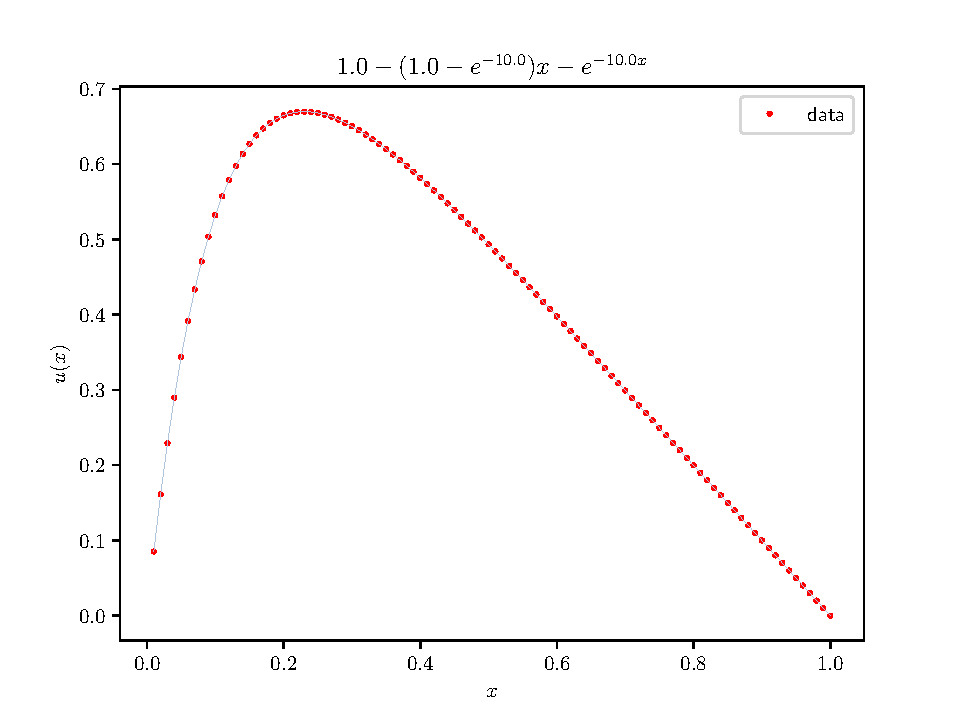
\includegraphics[scale=0.55]{../img/problem2-fig-x-u.pdf} %Imports the figure.
    \caption{Equation~\ref{eq:poisson_sol} is evalated at a descrete set of points shown in red. 
    The blue line has no significance and is only a visual aid.}
    \label{fig:problem2-fig-x-u}
\end{figure}
\begin{list}{}{}
    \item[$\bullet$] The C++ program \texttt{problem2.cpp} in the github repository is a basic
          program consisting of three functions: a function to generate and return
          the $x$ array, a function to evaluate equation~\ref{eq:poisson_sol} at each $x$ value and return 
          the $u(x)$ array and the main function which calls the former and writes the results to a file.
    \item[$\bullet$] The Python program \texttt{problem2.py} in the github repository is used
          to read the data file produced by the C++ program and plot the data using \texttt{matplotlib}.
          The resuling plot is shown in figure~\ref{fig:problem2-fig-x-u}.  
\end{list}

Next up is a table, created using the \texttt{table} and \texttt{tabular} environments. We refer to it by table \ref{tab:output_table}.
\begin{table}%[h!]
    \centering
    \begin{tabular}{c@{\hspace{1cm}} c}
        \hline
        Number of points & Output \\
        \hline
        10 &  0.3086\\
        100 &  0.2550\\
        \hline
    \end{tabular}\caption{Write a descriptive caption here, explaining the content of your table.}\label{tab:output_table}
\end{table}

Finally, we can list algorithms by using the \texttt{algorithm} environment, as demonstrated here for algorithm \ref{algo:midpoint_rule}.
\begin{algorithm}[H]
    \caption{Some algorithm}\label{algo:midpoint_rule}
    \begin{algorithmic}
        \State Some maths, e.g $f(x) = x^2$.  \Comment{Here's a comment}
        \For{$i = 0, 1, ..., n-1$}
        \State Do something here 
        \EndFor
        \While{Some condition}
        \State Do something more here 
        \EndWhile
        \State Maybe even some more math here, e.g $\int_0^1 f(x) \dd x$
    \end{algorithmic}
\end{algorithm}
   
\end{document}

